\documentclass[tikz, margin=0.1pt]{standalone}
\usepackage{tikz} 

\begin{document}

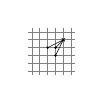
\begin{tikzpicture}[scale=1, dot/.style = {circle, fill, minimum size=#1, inner sep=0pt, outer sep=0pt}, dot/.default = 1pt] 

\foreach \y in {0.4,0.5,...,1} {
  \draw[gray, very thin] (.35,\y) -- (.95,\y);
}

\foreach \x in {0.4,0.5,...,1} {
  \draw[gray, very thin] (\x,0.35) -- (\x,.95);
}

% Start 
\draw[very thin] (0.8,0.8) +(0.02,0.02) -- +(-0.02,-0.02);
\draw[very thin] (0.8,0.8) +(-0.02,0.02) -- +(0.02,-0.02);

% Dots 
\node[dot] at (0.7, 0.7) {};
\node[dot] at (0.7, 0.6) {};
\node[dot] at (0.6, 0.7) {};


% Lines
\draw[very thin] (0.8, 0.8) -- (0.7, 0.7); 
\draw[very thin] (0.8, 0.8) -- (0.7, 0.6);
\draw[very thin] (0.8, 0.8) -- (0.6, 0.7);


\end{tikzpicture}

\end{document}
    
